% !BIB program = bibtex

\documentclass[12pt,letterpaper]{article}
\usepackage[utf8]{inputenc}
\usepackage[T1]{fontenc}
\usepackage{amsmath}
%\usepackage{amsfonts}
%\usepackage{amssymb}
\usepackage{makeidx}
\usepackage{graphicx}
\usepackage[normalem]{ulem}
\usepackage[singlespacing]{setspace}
\usepackage{subcaption}
\usepackage{float}
\usepackage{longtable}
\usepackage{multirow}
\usepackage{titlesec}
\setcounter{tocdepth}{2}
\usepackage[margin=1in]{geometry}
\usepackage{ntheorem}
\usepackage{booktabs}
\usepackage{dcolumn}
\usepackage[stable]{footmisc}

% font
\usepackage[charter,cal=cmcal]{mathdesign}

\usepackage{ntheorem}
\newtheorem{hyp}{Hypothesis}
\newtheorem{subhyp}{Hypothesis}[hyp]
\renewcommand\thesubhyp{\thehyp.\alph{subhyp}}
\usepackage{tikz}
\usetikzlibrary{arrows, decorations.pathmorphing, backgrounds, fit, positioning, shapes.symbols, chains, decorations.pathreplacing}
\usepackage[round]{natbib}
\bibpunct{(}{)}{;}{a}{}{,~}
\usepackage[space]{grffile}
\graphicspath{{./figures/}}
\usepackage[affil-it]{authblk}
\makeatletter

\def\@maketitle{%
	\newpage
	\null
%	\vskip 2em%
	\begin{center}%
		\let \footnote \thanks
		{\Large\bfseries \@title \par}%
		%\vskip 1.5em%
		{\normalsize
		%	\lineskip .5em%
			\begin{tabular}[t]{c}%
				\@author
			\end{tabular}\par}%
		%\vskip 1em%
		{\normalsize October 23, 2018}%
	\end{center}%
	\par
	%\vskip 1.5em
	}
\makeatother

\title{Friends Without Benefits: Explaining Costly Contributions to Unnecessary Wartime Coalitions}

\author{J Andr\'{e}s Gannon%
	\thanks{Electronic address: \texttt{jagannon@ucsd.edu} Web: \texttt{jandresgannon.com}}}
\affil{Department of Political Science \\ University of California, San Diego}

\author{Daniel Kent%
	\thanks{Electronic address: \texttt{kent.249@osu.edu} Web: \texttt{dnkent.github.io} \\ Draft version, please do not circulate. We thank the Center for Peace and Security Studies (cPASS), in particular Erik Gartzke, Rex Douglass, Matthew Millard, Michael Rubin, Thomas Scherer, and Alexandra Woodruff for their comments and suggestions and also thank Erin Ling, Amanda Madany, Cole Reynolds, Effie Sun, Erin Werner, and Lisa Yen for excellent research assistance. We also thank panel participants at the 2018 American Political Science Association conference, especially Camber Warren, for feedback. This research was sponsored by Office of Naval Research Grant N00014-14-1-0071 and the Department of Defense Minerva Research Initiative. Any opinions, findings, and conclusions or recommendations expressed in this publication are those of the authors and do not necessarily reflect the view of the Office of Naval Research.}}
\affil{Department of Political Science \\ The Ohio State University}

\begin{document}
\maketitle

\begin{abstract}
What determines the degree of alliance contributions to conflict theaters? France's military budget was twice the size of Italy's at the outbreak of the Gulf War, yet their troops contribution was ten times the size. This disparity demonstrates a simple but consequential point: alliance commitments are always unequal. We shed light on this important but under-explored topic by exploring the determinants of the degree of alliance contributions to conflict theaters. Through a new data set of relative country-level military contributions to the war in Afghanistan (2001-2014), we measure the extent to which states committed troops to the war during its early years, relative to how many troops they could have contributed. Drawing upon measures of position within the alliance network we argue that states contribute to ongoing conflicts in proportion to their potential gains in the broader security community. Countries that are already closely aligned with the central coalition actors and those stranded on the periphery alike tend to under-commit troops relative to the largest contributors, whose moderate alignments leave substantial room for subsequent gains to be had from signaling their commitment to the leading coalition actor.
\end{abstract}

\doublespacing
\section{Introduction}
	In 2001 the United States launched the war in Afghanistan with the goal of overthrowing the Taliban and dismantling Al Qaeda. But it did not do so alone; instead it led a coalition of 50 other states that fought alongside the United States until it formally ended in 2014.\footnote{This refers to Operation Enduring Freedom, not the ongoing Operation Freedom's Sentinel, which has been conducted far more unilaterally.} Not every state contributed equally. While the United States sent thousands of troops for the duration of the conflict, others contributed only a handful to fulfill their contractual alliance obligations under NATO. Yet some state had no formal alliance obligations and still sent troops in a manner that risked significant costs for that state. New Zealand lost almost a dozen troops in the Afghanistan conflict; a difficult thing for a state leader to justify to their public when the outcome of the conflict is largely immaterial to the state at hand.

This is exemplary of a broader trend in coalition warfare. Some states contributes forces to coalition wars because they care about the material outcome of the conflict and hope to influence that outcome in some significant way. Others contribute forces because alliance obligations or expectations create a cost to free riding. But neither of those theories explain contributions like that of New Zealand to the war in Afghanistan; states that are unaffected by the outcome of the conflict, that have no notable ability to influence the outcome of the war, that experience no reputational cost from refusing to participate, and yet willingly risk high costs from their participation. Table \ref{table:2001_top} shows that New Zealand is not an isolated incident. Many of the states that made the most personally costly contributions were not those that had the largest stake in the outcome.

	\vspace{-4em}

		\begin{quote}
		\begin{table}[ht]
			\centering
			\begin{tabular}{|lr|}
				\hline
				\textbf{State} & \textbf{Contribution} \\
				\hline
				Denmark & 0.66 \\
				New Zealand & 0.65 \\
				United States & 0.53 \\
				Romania & 0.53 \\
				Netherlands & 0.44 \\
				Germany & 0.44 \\
				Norway & 0.34 \\
				Australia & 0.29 \\
				Turkey & 0.27 \\
				Spain & 0.20 \\
				\hline
			\end{tabular}
		\caption{Top 10 contributors to ISAF (2001) by percent of armed forces. Source: IISS Military Balance, 2002. Canada's conflict-leading contributions are omitted because this data only references 2001.}
		\label{table:2001_top}
		\end{table}
		\end{quote}

	This paper explains such contributions by developing a new theory about coalition warfare participation by states whose primary objective in fighting is not to influence the outcome of the conflict or maintain their current reputation as reliable allies who fulfill their contractual obligations. We develop a new theory of states who contribute forces to coalition warfare in order to \textit{develop} their reputation as reliable allies because their contribution is disproportionately costly relative to the size of their armed forces. We find that if state military contributions are measured not by the number of troops they contributed, but the proportion of their military forces they contributed, that states seeking to develop a stronger relation with the central actor in the coalition network are more likely to have higher proportional troop contributions.

	In other words, states that wish to increase their ties to central actors in the coalition network seek to do so by over-contributing, sending a larger portion of their armed forces than other states that were formally obligated to partake in coalition operations. This finding has important implications for understanding the costly means by which states seek to re-align themselves in international alliance networks. Conflict is generally understood as a costly tool which states employ to achieve their international objectives. One of those objectives can be unrelated to the outcome of the conflict itself. States may rely on war efforts to serve as a signal of willingness to undergo large costs in the hopes that this will improve their relationship with central states in the future. This can help explain the ways that states use conflicts which are not of immediate strategic importance to gain the attention and (hopefully) respect of central players in the international system. Simply put, war can be a good excuse for improving ties with important states.

	This paper proceeds in five parts. In part two we explore existing explanations for coalition warfare, which thus far have focused on the manner in which states fight together rather than explaining why they bother fighting together at all. Part three develops our theory by applying the costly signaling theory to coalition warfare through a novel measure of the costliness of a state's contribution to coalition warfare: the relative pressure of that mobilization based on the size of its available armed forces. Part four empirically test this finding by examining coalition contributions during the war in Afghanistan (2001-2014), which presents a ripe test case for our theory given variation in the alliance obligations of the states that participated as well as their level of participation. Section five includes a discussion of the generalizability of our results for the broader theory, explaining how states seek to alter and leverage their position within the network of capable international actors. Section six concludes and discusses areas where we are particularly interested in receiving feedback.

\section{Existing Explanations for Contributions to Coalition Warfare}
	Attempts to explain why countries contribute to alliances can be divided into four different categories; theories of collective action, the balance of threat, alliance dependence, and domestic politics \citep{bennett_burdensharingpersiangulf_1994, haesebrouck_democraticparticipationair_2016}. The \textit{collective action hypothesis} introduced by \citet{olson_economictheoryalliances_1966} argued that dominant states will end up making the largest contributions because smaller states can simply free ride while continuing to garner the benefits of the alliance relationship writ large. These dominant states, with larger economies and militaries, end up paying a disproportionate burden to secure goods even when the public benefits of those goods are reaped by states that made little contribution themselves. The \textit{balance of threat hypothesis} argues that state contributions should be proportional to the gravity of the threat an issue presents to a state. When faced with a larger threat, a state will contribute more to an alliance coalition that they anticipate mitigating that threat \citep{walt_originsalliance_1987, sandler_natoburdensharing_2014, baltrusaitis_coalitionpoliticsiraq_2010}. The \textit{alliance dependence hypothesis} argues that states in an alliance must balance two competing fears; the fear of abandonment and the fear of entrapment \citep{snyder_securitydilemmaalliance_1984}. Problematically, reducing one of these risks necessitates an increase in the risk of the other. Allied support is thus explained by how a state feels about these relative risks; a states will contribute to an alliance when the fear of abandonment exceeds the fear of entrapment. States that most fear abandonment will be those that are most dependent on the other partner in the alliance meaning the military and economic payoffs of the alliance relationship would be difficult to replace. This theory has been expanded by scholars who note that ``alliance value" explains contributions by states who believe they can leverage their allies partner in their favor \citep{davidson_neoclassicalrealistexplanation_2011}. The \textit{domestic hypotheses} of alliance contributions take multiple forms \citep{ashraf_politicscoalitionburdensharing_2011}. Theories of state autonomy and domestic society predict that leaders that can insulate themselves from external constraints on their decision-making about alliance contributions are consequently able to do so even when these leaders' preferences regarding contributions differ from those of the public \citep{saideman_ambivalentcoalitiondoing_2016, vonhlatky_ideologyballotsalliances_2018}. Theories of bureaucratic politics instead examine the relationship within the government. Bureaucratic decision-making requires negotiations and bargaining among relevant actors and as such state contributions are the outcome of these bargaining decisions and the the environment shaping the bargaining framework \citep{mello_democraticparticipationarmed_2014, rathbun_partisaninterventionseuropean_2004}.

	Other literature on state contributions to joint efforts have examined topics like UN peacekeeping. Here, research has found that states that are more centrally located within the international network as measured by policy preferences will contribute the most troops to that peacekeeping mission because they gain private benefits from fighting alongside like-minded states \citep{dorussen_networkedinternationalpolitics_2016}. While theoretically important, these findings do not explain the costliness of a state's contribution nor whether that contribution was used as a signal to improve a state's ties with other actors in the network. Their network position is assumed as a static factor explaining the level of contribution when in reality it is a position that states want to actively manipulate. The costliness of UN peacekeeping contributions as a signal is harder to measure considering the risk of casualties and collateral damage is lower and domestic publics are less attuned to their state's participation in UN peacekeeping than active military operations.

\section{Theory of Signaling via Coalition Contributions}
	\subsection{Relative Contribution Cost and Dynamic Interstate Alliances}
		While most of the recent research on contributions to coalition warfare has focused on explaining the magnitude of state contributions, the foundational literature argued that support for all four theories was empirically observed because they explained different phenomena. External pressures like collective action, the balance of threat, and alliance dependence explain \textit{whether} a state contributes to coalition warfare but \textit{how} that state contributes has been argued to be explained by internal constraints \citep{bennett_burdensharingpersiangulf_1994}. The problem throughout much of this previous work is in how it measures the size of a state's contribution. Almost all prior analysis has measured a state's contribution in absolute terms; the number of troops, financial contributions, foreign aid, or peacekeepers sent a particular operation \citep{mello_democraticparticipationarmed_2014, haesebrouck_explainingmemberstates_2016}. This measure makes sense for theories interested in explaining who contribute the most, since absolute terms describe the highest contributors. But this does not describe the expected cost a state faces for making a contribution. It is less costly for the United States to send 1,000 forces into a conflict theater than for Poland to do the same. The former has a substantially larger military force and thus experiences a lower national cost in terms of the burden such a contribution places on its military forces and the zero-sum trade-off of this contribution relative to other security needs. Figure \ref{fig:contrib_map} shows that these two measures -- total troops contributed and percent of troops contributed -- provide different baselines about which states had the most costly contributions to the war in Afghanistan.

		\begin{figure}[H]
			\centering
			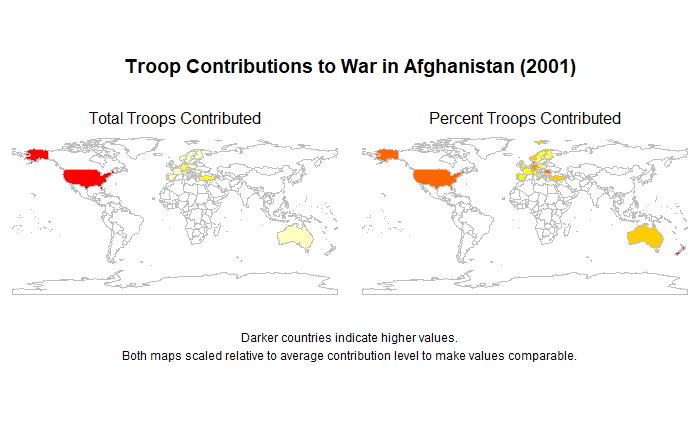
\includegraphics[width=\textwidth]{troops_2001_sidebyside_scaled.png}
			\caption{Country Troop Contributions to war in Afghanistan (2001) Source: IISS Military Balance report}
			\label{fig:contrib_map}
		\end{figure}

		The second problem is how current hypotheses think about alliances. These theories anticipate the highest contributions coming from states that are dependent on the security guarantee of the central coalition actor and those that perceive a special relationship with the United States \citep{haesebrouck_democraticparticipationair_2016, howorth_securitydefencepolicy_2014, graeger_revivalatlanticismnato_2009, biehl_strategiccultureseurope_2013}. However, this views the alliance relationship as temporally indistinct and oriented towards maintaining continuity in the current relationship, not seeking change. As such, the assumption is that countries that fight together do so because they already have closely aligned interests. What this misses is how fighting together can be a method for altering the perceived alignment of interests.

	\subsection{Benefits of Over-contributing Forces}
		We argue that a state can use over-contributions to coalition warfare as a costly signal to the central coalition actor that it desires a closer relationship with that central actor. Over-contributing is a way to send a separating signal that even though a state may be less closely aligned with the central actor prior to or at the outset of the conflict, it is willing to incur costs for the benefit of the central actor.

		A few factors must be true for this theory to hold. First, the over-contributing state must not be seen as participating in the conflict because it garners security benefits from the conflict's outcome. If this were the case, the central coalition actor would be less likely to interpret the over-contribution as a sign of good will and would instead interpret it as self-interest. Second, the over-contributing state must be dissatisfied with the current state of the alliance relationship. While the current alliance hypotheses argues that the highest contributions will come from states that have a special relationship with the United States or that are currently dependent on the security guarantee, we argue instead that states that would benefit from an increased security dependency or that want a more tightly linked relationship with the United States will have more costly contributions. States that already have a special relationship or a reliable security guarantee do not need to over-contribute because their relationship is, in some sense, locked in. These states have some flexibility in their expected contributions and are unlikely to lose their special relationship status simply because they did not go above and beyond in contributing to the coalition effort. They just need to contribute enough that they are not seen as free riders.

		Rather, states will over-contribute to coalition warfare when they expect their contribution to serve as a costly signal of their expectations for future alliance value. This differs importantly from the ``alliance value" explanation provided by \citet{davidson_americaallieswar_2011} and \citet{massie_democraticalliesfollowership_2016} who hypothesize that it's about present alliance value. States with a high, but stable current alliance value have no incentive to over-contribute because they don't get any additional payoff from doing so and there is a lower risk of fallout from making a normal contribution since their ties are already close \citep{davidson_headingexitsdemocratic_2014}. This is why small states are able to free ride and take the relationship for granted as pointed out by \citet{keohane_biginfluencesmall_1971} but we don't always see that because those that desired an improved tie won't free ride and will in fact try to signal the opposite. In these cases, you have less of a need to signal your value for the relationship than when you are acquaintances that would benefit from signaling a change in your desired alignment tie \citep{gartzke_contractsfriendsalliances_2012, gibler_priorcommitmentscompatible_2004}.

		\begin{hyp}
			A state with an interest in improving relationship ties with the central coalition actor will make more costly contributions than a state without an interested in improving relationship ties.
		\end{hyp}

		Our theory, presented in figure \ref{fig:theory}, thus predicts a non-linear relationship between the current strength of a state's alliance with the central coalition actor and that state's expected cost of contributing to the coalition war effort. Previous work about alliances expects this relationship to be linear \citep{massie_democraticalliesfollowership_2016, haesebrouck_explainingmemberstates_2016, ringsmose_natoburdensharingredux_2010}. The closest allies of the central coalition actor may make the highest absolute contributions by virtue of their size and military strength, but they are not the states that make the highest relative contributions since they have no incentive to incur the costs that high relative contributions entail. Instead, it's those that want to be closer allies, relatively speaking, that contribute the most.

			\begin{figure}[H]
				\centering
				\begin{tikzpicture}
				% Graph axes
				\draw[thick,<->] (0,5) node[above]{Expected Cost of Contribution} -- (0,0) -- (8,0) node[right]{Relationship Tie Strength};

				% Contribution Curve
				\draw[thick] (0,0)..controls (5,5) ..(8,2.5);

				% Desired Relationship Tie
				\draw[dashed] (4,0) -- (4,3.5);
				\draw[dashed] (6.5,0) -- (6.5,3.5);
				\draw[decorate,decoration={brace,mirror,raise=5pt}, thick]
				(4,0) -- (6.5,0);
				\node at (5.25,-0.7) {Desire Improved Tie};
				\end{tikzpicture}
				\caption{Theory of State Contributions to Wartime Coalitions}
				\label{fig:theory}
			\end{figure}

		%The primary benefit a state gets from an alliance are its security benefits since states are able to aggregate capabilities in a way that increases their protection against foreign threats \citep{waltz_theoryinternationalpolitics_1979}.
		Though there is an extensive literature on the ways in which states aggregate their capabilities to bolster their security against foreign threats \citep{waltz_theoryinternationalpolitics_1979}, the security benefits of an alliance do not precisely map onto the security benefits of joining a wartime coalition. The former is an example of a public good; the benefits of the alliance can be reaped even if a participant in the alliance free rides \citep{olson_economictheoryalliances_1966}. During wartime coalitions, however, there are more clear private benefits to states from participating in that coalition. Advocates of the balance of threat perspective point to private incentives actors have to ensure that the aggregate contributions to defense are sufficient to deal with the threat \citep{bennett_friendsneedburden_1997, baltrusaitis_coalitionpoliticsiraq_2010, davidson_neoclassicalrealistexplanation_2011}. 		States get private good benefits from coalition war-fighting. For some states, that private good is a desirable war outcome.  For others, the private good to be gained from coalition war-fighting is improving the quality of your relational tie with the central actors leading that conflict. This tie is most improved when a state's contribution to the coalition effort is a costly signal of their commitment to the conflict which happens when they have over-contributed relative to the contribution that would be expected from a state with their military capacity. Since alliances are a costly signal of one's intention to cooperate, it should also be true that fulfilling alliance-like obligations even when you are not bound by those alliance obligations would also be a signal of your desire to cooperate more in the future \citep{warren_geometrysecuritymodeling_2010}.

		Besides security, there are other reasons state seek and maintain alliances with other states. There are domestic benefits to establishing yourself as a closer ally with a powerful country as was witnessed with Egypt in the 1960's \citep{barnett_domesticsourcesalliances_1991} and the United Kingdom during the Iraq War \citep{davidson_americaallieswar_2011}. In these cases, political leaders who fear domestic opposition from other government actors like bureaucrats or non-partisans or from non-government actors like voters or interest groups may use alliances with other states to demonstrate competent policymaking.

		This private goods theory of coalition conflict, as distinct from alliances, explains why states would vary in the \textit{degree} of their contribution. Acquaintances make a costly contribution when they could have chosen to free ride because their interest is not in the public good of security achieved via victory in the conflict but private interests like a security umbrella down the road or closer economic or diplomatic ties with the state to whom they sent a costly signal of support. Previous literature has noted that you should get a payoff from signaling that you honored an alliance commitment and states that do so get more allies in the future because they are seen as reliable \citep{gibler_costsrenegingreputation_2008}. This is consistent with our logic where you hope that your signal of strongly valuing the relationship causes the other actor to later take actions that recognize that.

		Because the value of the signal is determined by its cost, not by its effect, it does not matter if the signaling state sends forces that can materially influence the outcome of the conflict \citep{davidson_americaallieswar_2011}. It only matters that the signal is interpreted as one that was costly for the sender irrespective of its effects. In most cases, the powerful state not only does not need support from smaller state in order to win the conflict, but may actually want to maintain control of the forces that will determine the conflict outcome. This is consistent with alliance theories about the autonomy benefits one actor gets from asymmetric alliances \citep{morrow_alliancesasymmetryalternative_1991}. As such, smaller states do not want to make contributions that are too influential in the conflict's outcome because of the risk of intruding upon the powerful state's decision-making. Importantly, this differs from other perspectives like \citet{bennett_burdensharingpersiangulf_1994} since the US is not exercising leverage over smaller states to induce their contributions, instead the momentum comes from the smaller states whose contribution does more to serve their interests than the interests of the powerful state.

\section{Research Design}
	\subsection{Data}
		Our dependent variable is country-year troops contributions to the war in Afghanistan. For the first model, we measure this as a binary variable coded 1 if the country-state contributed any military forces and coded 0 otherwise. The second model measures country-year contributions as a ratio of the count of troops contributed divided by the number of troops in that country-years armed forces. As such, the second dependent variable is a measure of the cost a state accepts for a given contribution. To focus on the decision to commit troops, as opposed to a country's resilience to casualties -- which are not necessarily synonymous -- we focus on the opening stage of the war from 2001-2005. The costliness of a state's contribution is measured using troop ratios as opposed to financial cost since the risk of casualties and collateral damage are two costs unique to personnel contributions that states are attentive to when deciding whether and to what extent they should participate in coalition warfare \citep{ringsmose_natoburdensharingredux_2010, chivvis_topplingqaddafilibya_2014, haesebrouck_natoburdensharing_2017}. The troop data was gathered from the International Institute for Strategic Studies' (IISS) annual ``Military Balance'' reports \citep{internationalinstituteforstrategicstudies_militarybalance_} which includes detailed information on every country's current military portfolio and overseas commitments. Not only does the Military Balance include the number of troops each country contributed to the War in Afghanistan, it also contains information on the total number of troops in each country's military at the time. Figure \ref{fig:afghan_total} shows the total number of troops in Afghanistan during the initial years of the war and figure \ref{fig:troop_hist} shows the distribution across states. Some states like Denmark, New Zealand, the United States and Romania contributed roughly 3 times the size of their armed forces than did the median contributor.

			\begin{figure}[H]
			\centering
				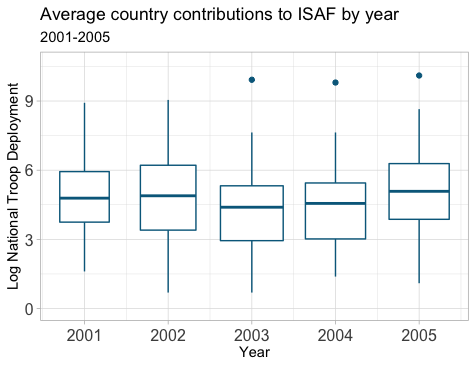
\includegraphics[width=0.5\textwidth]{figures/country_troop_boxplot.png}
			\caption{Total Foreign Troops in Afghanistan (2001-2005) Source: IISS Military Balance Report}
			\label{fig:afghan_total}
			\end{figure}

		Our explanatory variable is a state's relationship with the United States. We predict that states with moderate-strength relationship ties that desire improved ties will be more likely to choose costly contributions to signal that desire to the United States. We operationalize this using network statistics from the yearly alliance network. Also because of the potential benefits of signaling reliability to the United States, we compiled data on ideal point estimates relative to the United States in each year. Our primary network statistic of interest is a country's structural equivalence with the United States in the alliance network. This serves as a useful means of capturing the degree to which the country is deeply embedded within or sits on the periphery of the initiating state's security community.

			\begin{figure}[ht]
			\centering
				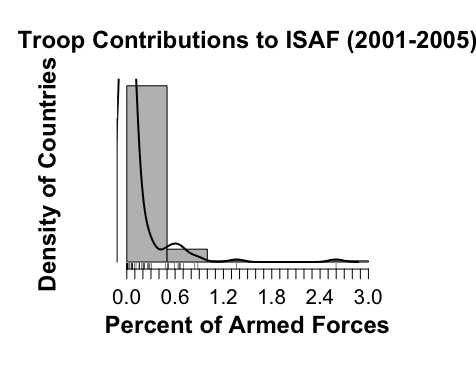
\includegraphics[width=0.5\textwidth]{figures/troops_hist_largebin.png}
			\caption{Distribution of Country Contributions to Afghan war (2001-2005) Source: IISS Military Balance report}
			\label{fig:troop_hist}
			\end{figure}

		As \ref{fig:contr_sequiv} demonstrates, the relationship between structural equivalence and troop contributions follows our expectation reasonably well, with a curvilinear relationship between a country's average contribution and their structural equivalence with the United States. However, it is important to note that the curvilinear relationship captures all countries well, except for Canada, who after 2002 actually contributed a far greater proportion of all troops \textit{and} is the most structurally equivalent country with the United States.\footnote{A figure including Canada is included in the appendix, to avoid too much clutter in the bulk of the paper. Feedback is especially appreciated here. We have no intention of leaving data out because it is inconvenient for our theory. But given the clear trend with all other countries, allowing one country to have so much leverage on a broader theory brings with it a new set of problems.} Throughout the rest of the paper, we fit all models with and without Canada to show that its inclusion includes substantial leverage on the conclusions reached, though in all other observations the hypothesized curvilinear relationship holds.


			\begin{figure}[H]
			\centering
				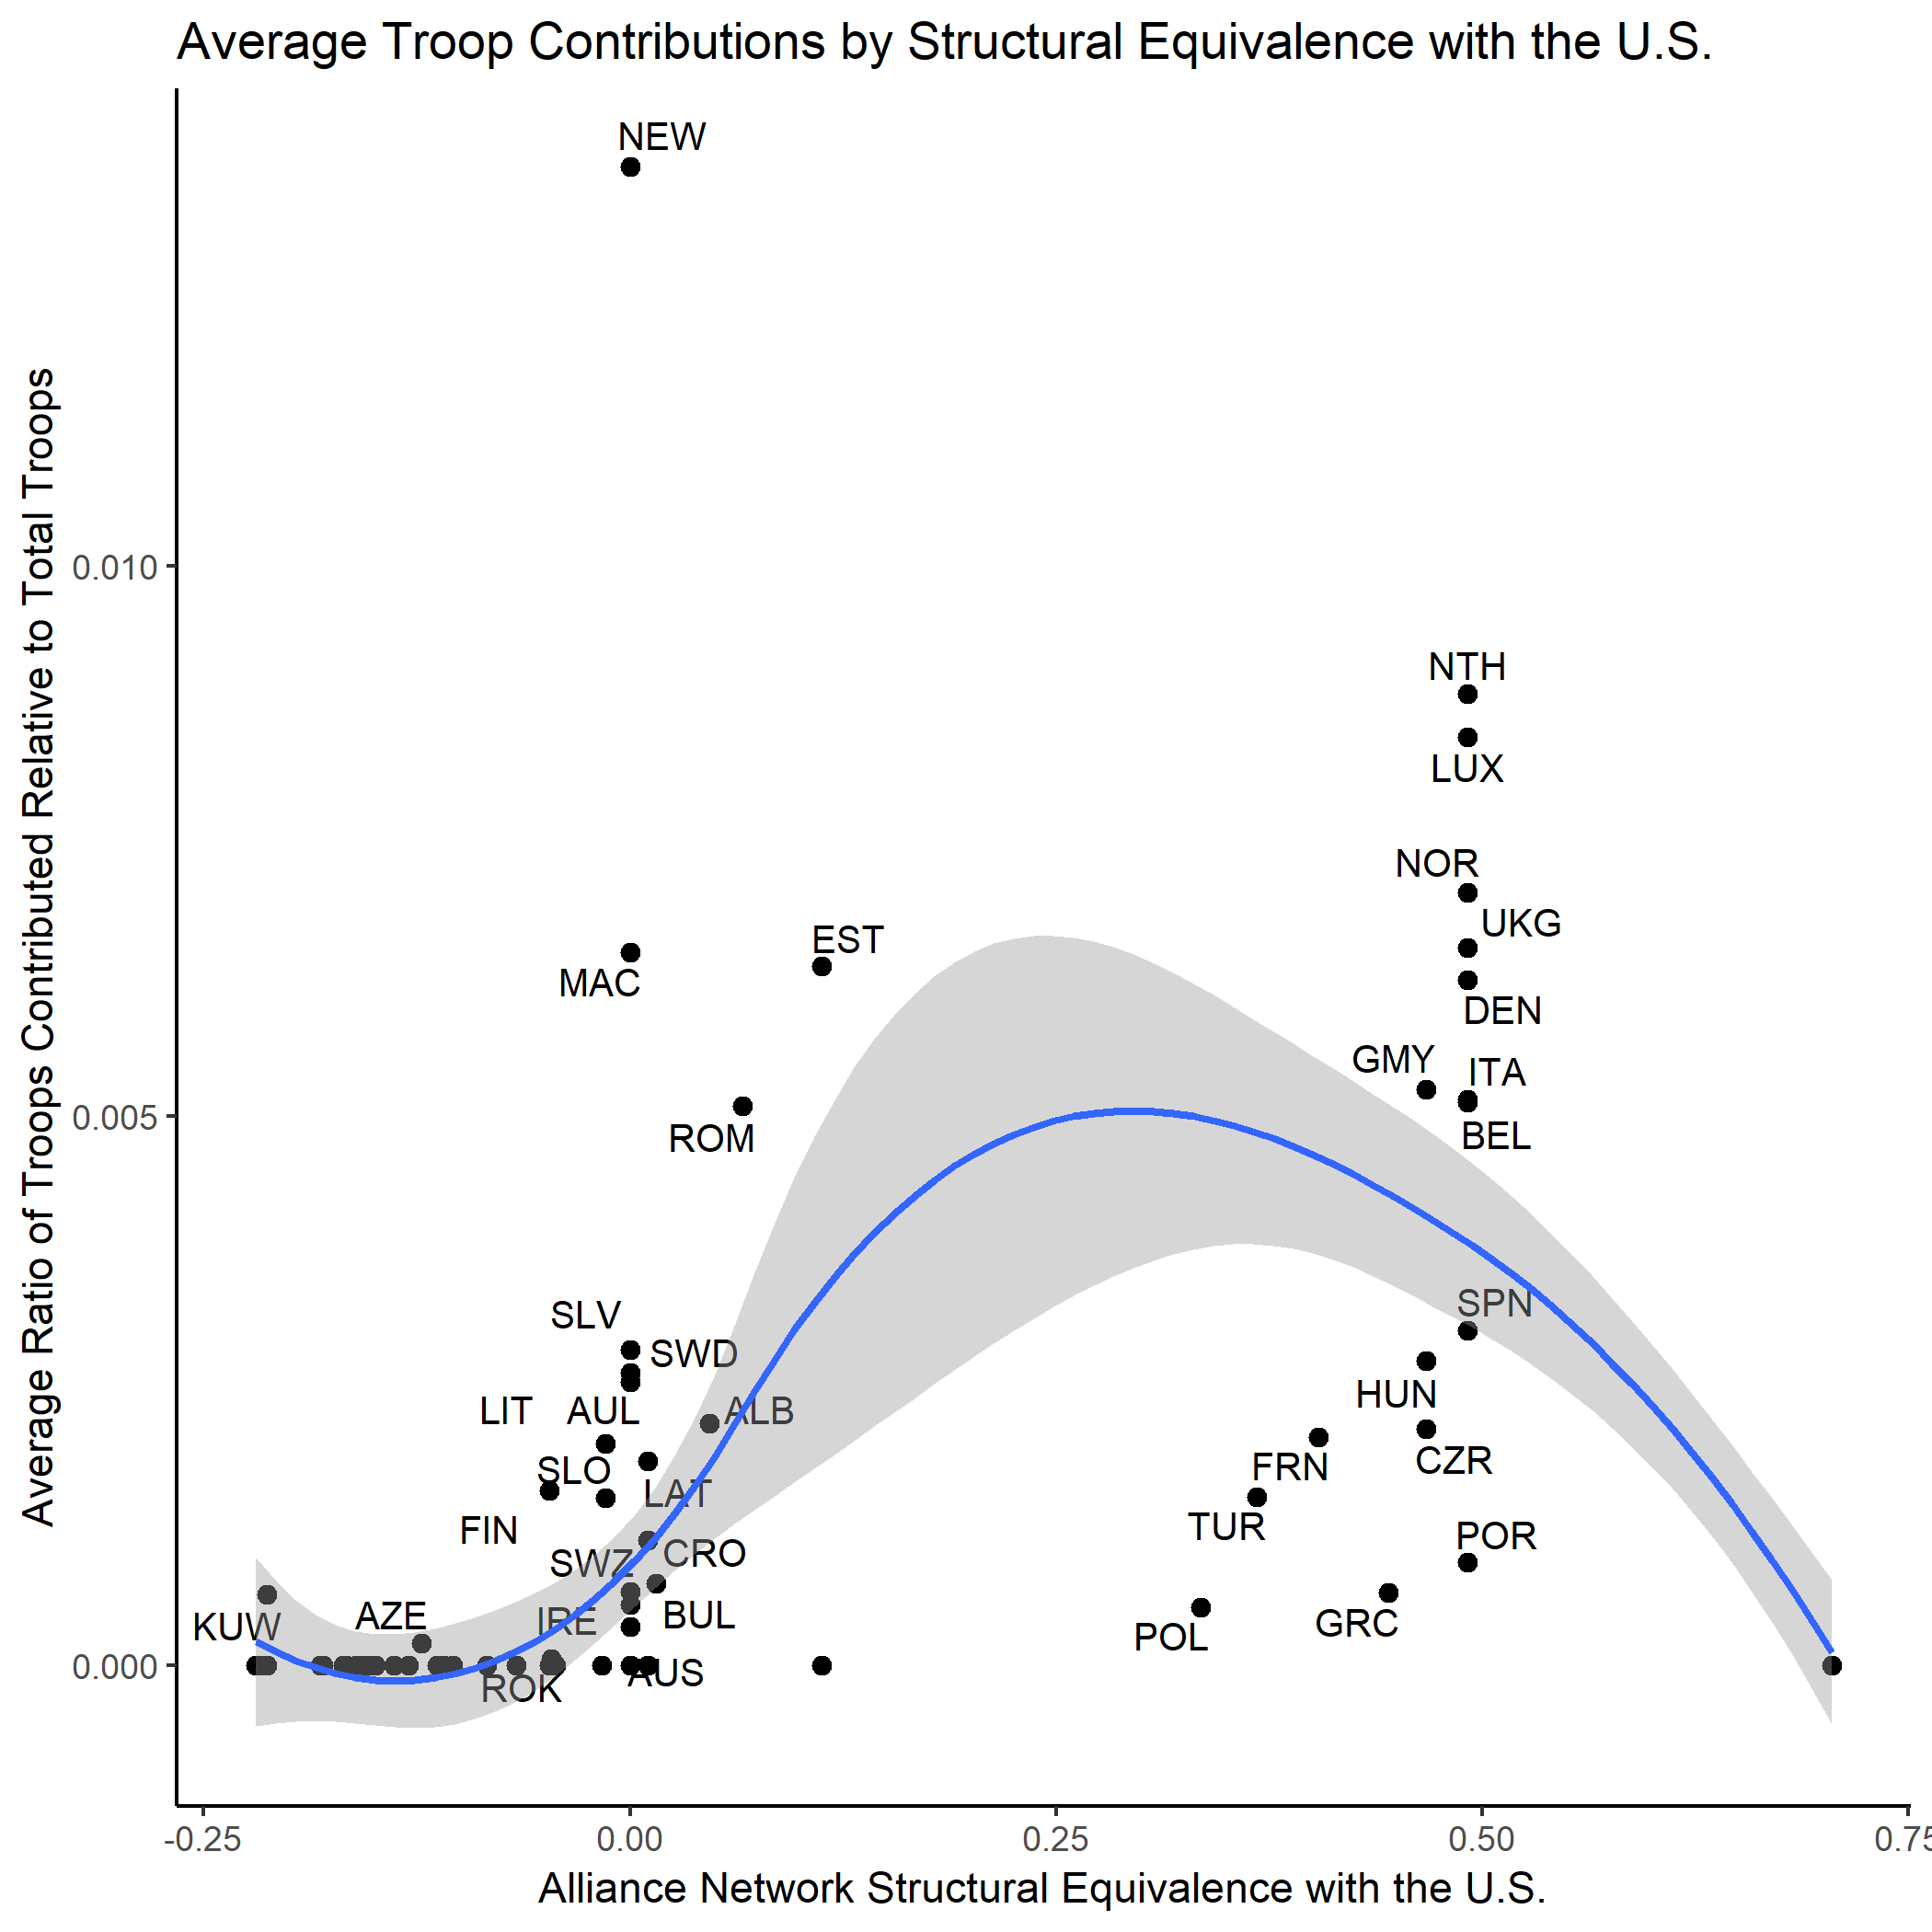
\includegraphics[width=0.55\textwidth]{figures/contributions.png}
			\caption{Troop Ratio by Structural Equivalence with the United States}
			\label{fig:contr_sequiv}
			\end{figure}

	\subsection{Models and Findings}
	Our unit of analysis for these models is the country-year, spanning from 2001-2005. Though we include and are primarily interested in measures of network statistics, because our outcome of interest is a node-level attribute, we employ generalized linear models and generalized additive models (GAMs) as opposed to methods for modeling tie formation (e.g. exponential random graph and latent space models).\footnote{We are also considering extensions of network models for node formation, i.e. \citet{fosdick2015}, at least as a robustness check of sorts. The only issue with the network approach being that said models are not designed to have the same effect flexibility as GAMs.} For each dependent variable, we estimate a baseline model focused only on effects of interest and then a second which includes controls for distance and democracy. In the former, we first fit a GLM with a polynomial term. But because a polynomial term forces a specific curvilinear relationship upon the data, we also fit a generalized additive model with smoothing terms to see if a similar relationship emerges under a less restrictive format.

		\subsubsection{Model 1: Decision to Commit Troops}
		The curvilinear relationship in figure \ref{fig:contr_sequiv} largely results from the data likely capturing two separate processes. First, capturing why the data is zero-inflated, states initially decide whether or not they will contribute any troops. In this section we model that choice, leaving the amount of troops provided for the next part. Our model for sending troops is represented by equation (1), where `equiv' represents structural equivalence in the alliance network with the United States\footnote{There are multiple possible measures of structural equivalence. We draw upon the Pearson coefficient, which compares the number of actual shared numbers to that one would expect in a truly random network.}. A state's distance from the U.S. in terms of its ideal point estimate is captured by `ideal'. \citep{bailey_twodimensionalanalysisseventy_2018} Last we include terms controlling for democracy and the state's distance from Afghanistan.

		%% Note I've dropped centrality (density) because it is multicollinear with structural equivalence
			\vspace{-2em}
			\begin{equation}
				\text{Contribution}_{it} = \beta_0 + \beta_1\text{equiv}_{it} +  \beta_2\text{ideology}_{it} + \beta_3\text{dem}_{it} + \beta_4\text{dist}_{it}
			\end{equation}

			\begin{figure}[H]
				\centering
					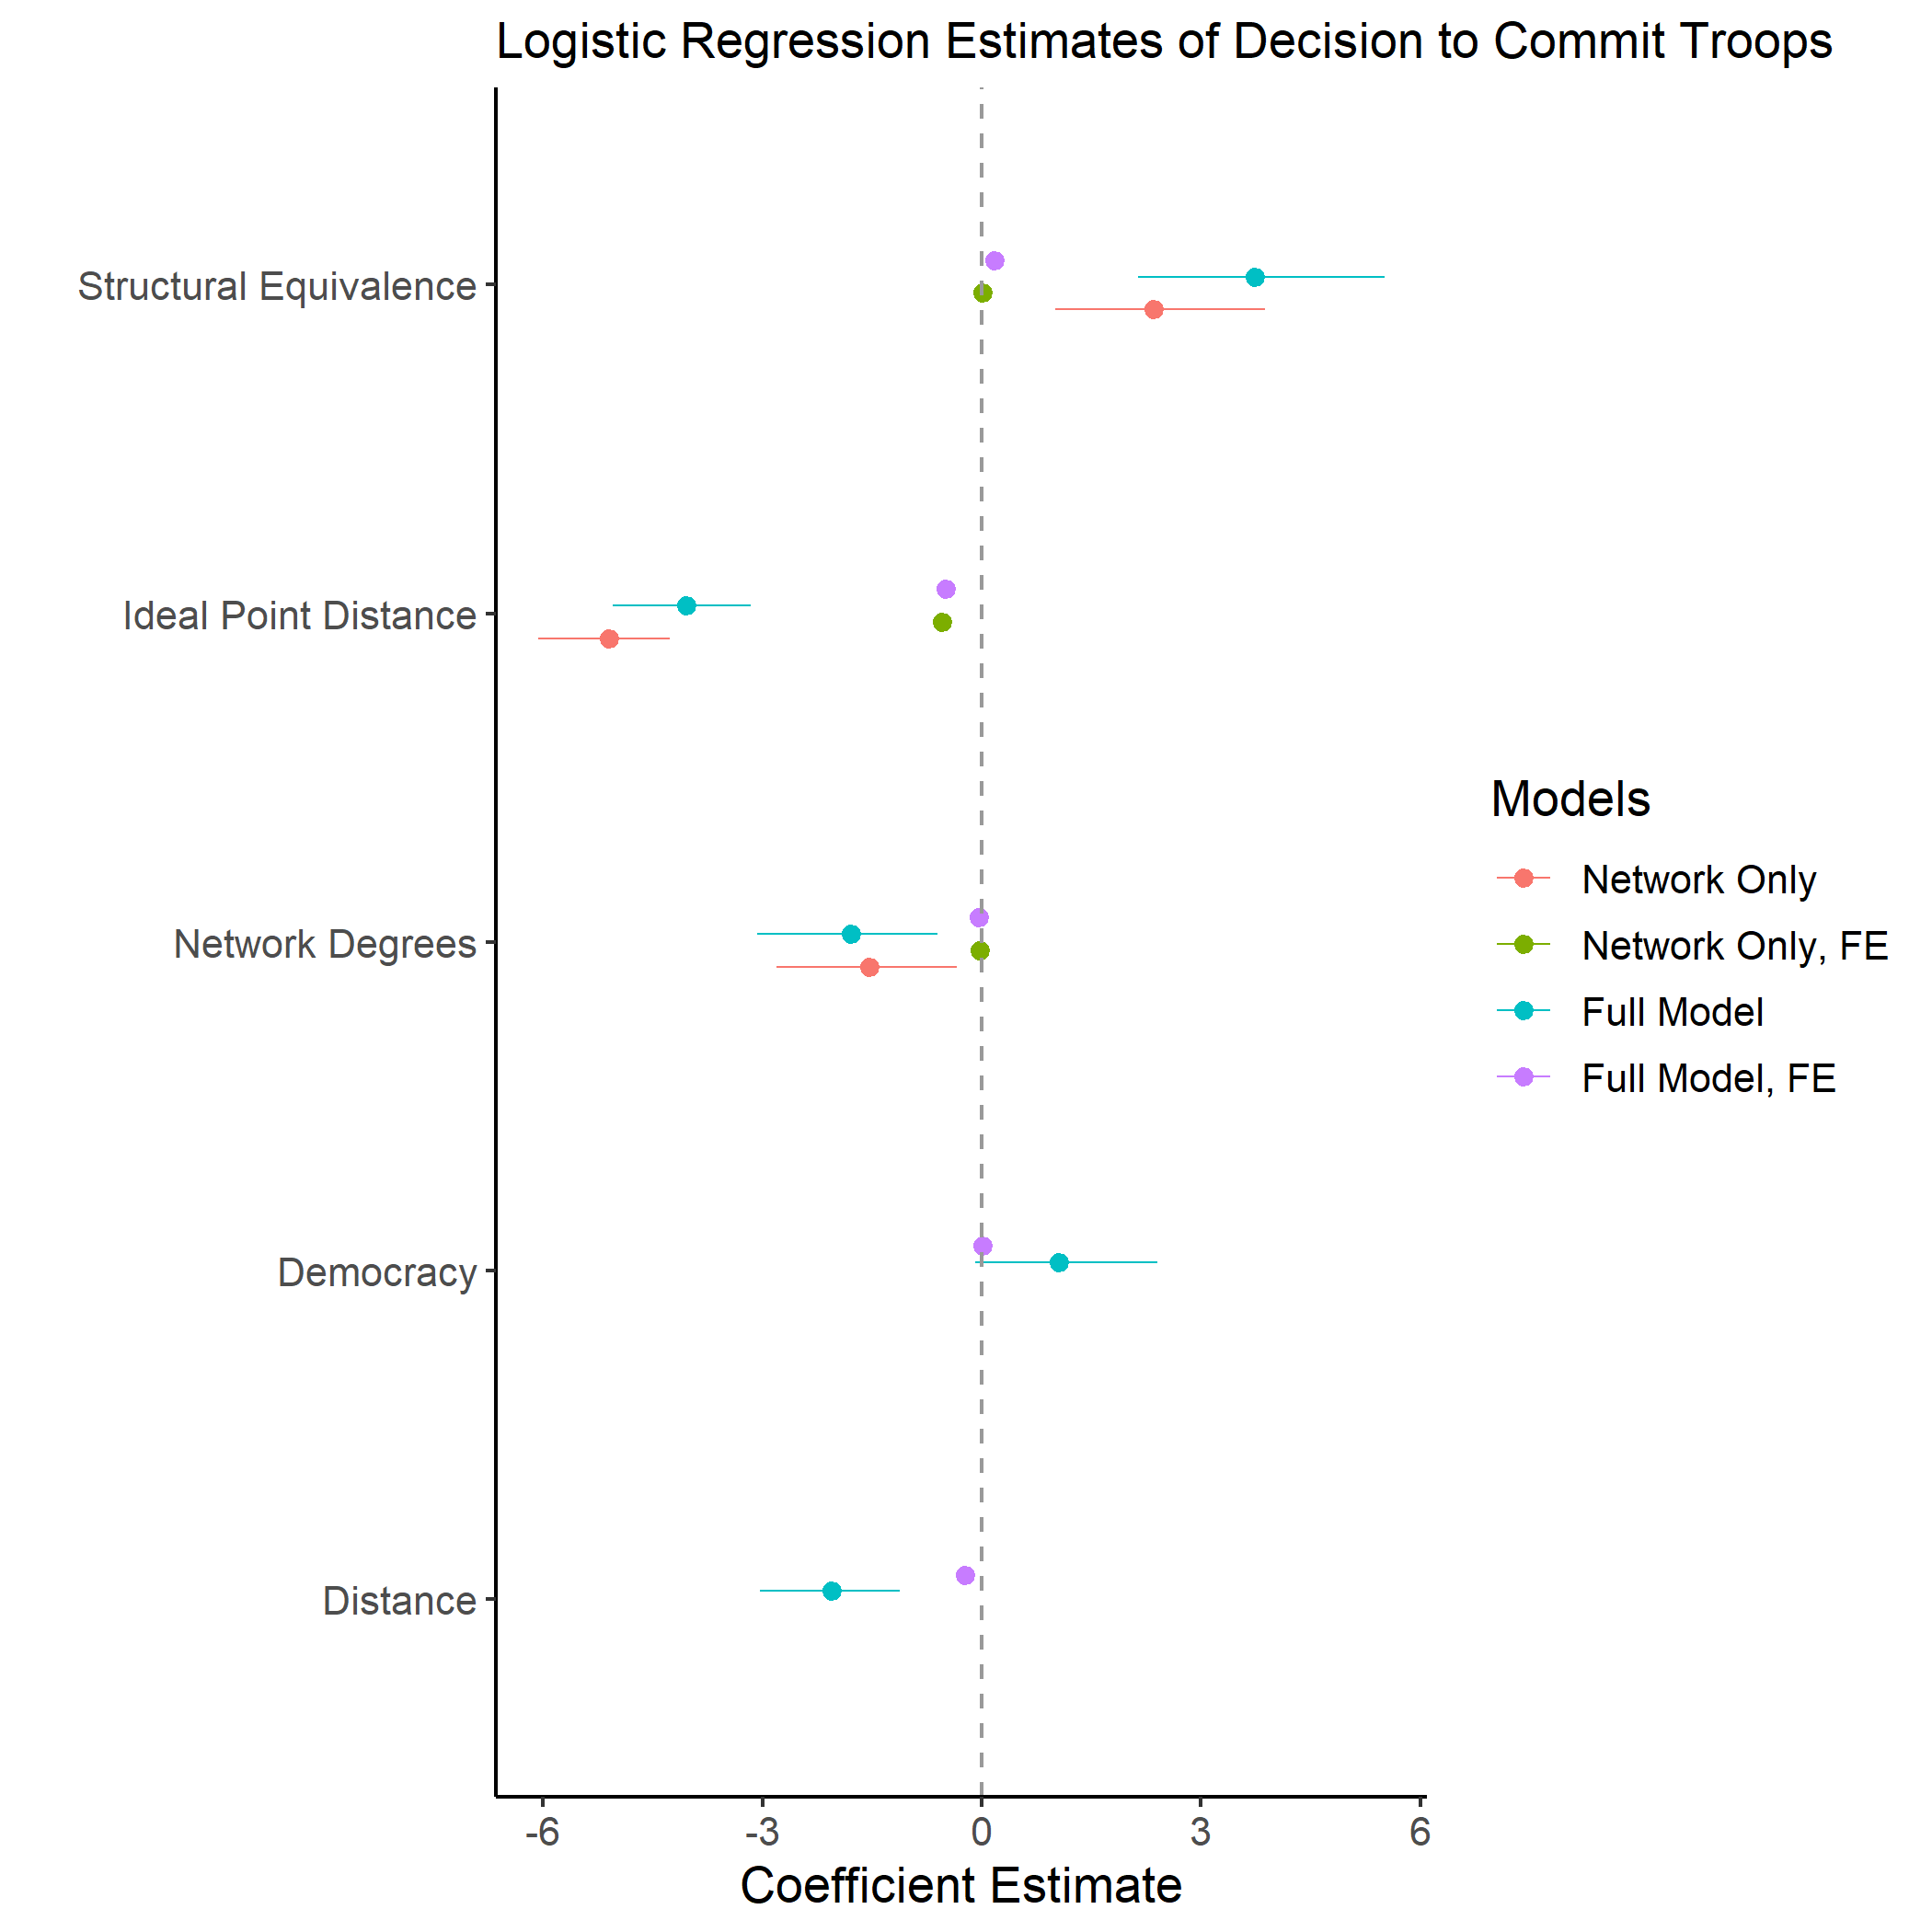
\includegraphics[width=0.725\textwidth]{logit_coef.png}
				\caption{Model 1: Decision to commit any troops. FE corresponds to fixed effects.}
				\label{fig:logit_reg}
			\end{figure}

		With respect to a state's decision to commit any troops to Afghanistan, we see that estimates for structural equivalence and ideal point distance are robust to specification and move in the expected directions. In particular, when it comes to the decision to commit troops at all, we see that ideological similarity with the United States is particularly powerful as a predictor. Figure \ref{fig:logit} demonstrates that the relationship is quite clear, with almost all contributors sitting close to the United States ideologically. Moreover, the predicted probabilities, which we derive from our logistic regression estimates, map on relatively cleanly to the actual data. However, it is important to note that our theory is focused on the \textit{amount} of troops contributed, meaning the curvilinear relationship corresponds to the next set of models.
		%However, it is important to note that the cluster of states which contribute are not those perfectly aligned with the US, but those closely aligned -- meaning they have room to gain from subsequent cooperation and, presumably, grow closer, as our theory expects.

			\begin{figure}[H]
			\centering
				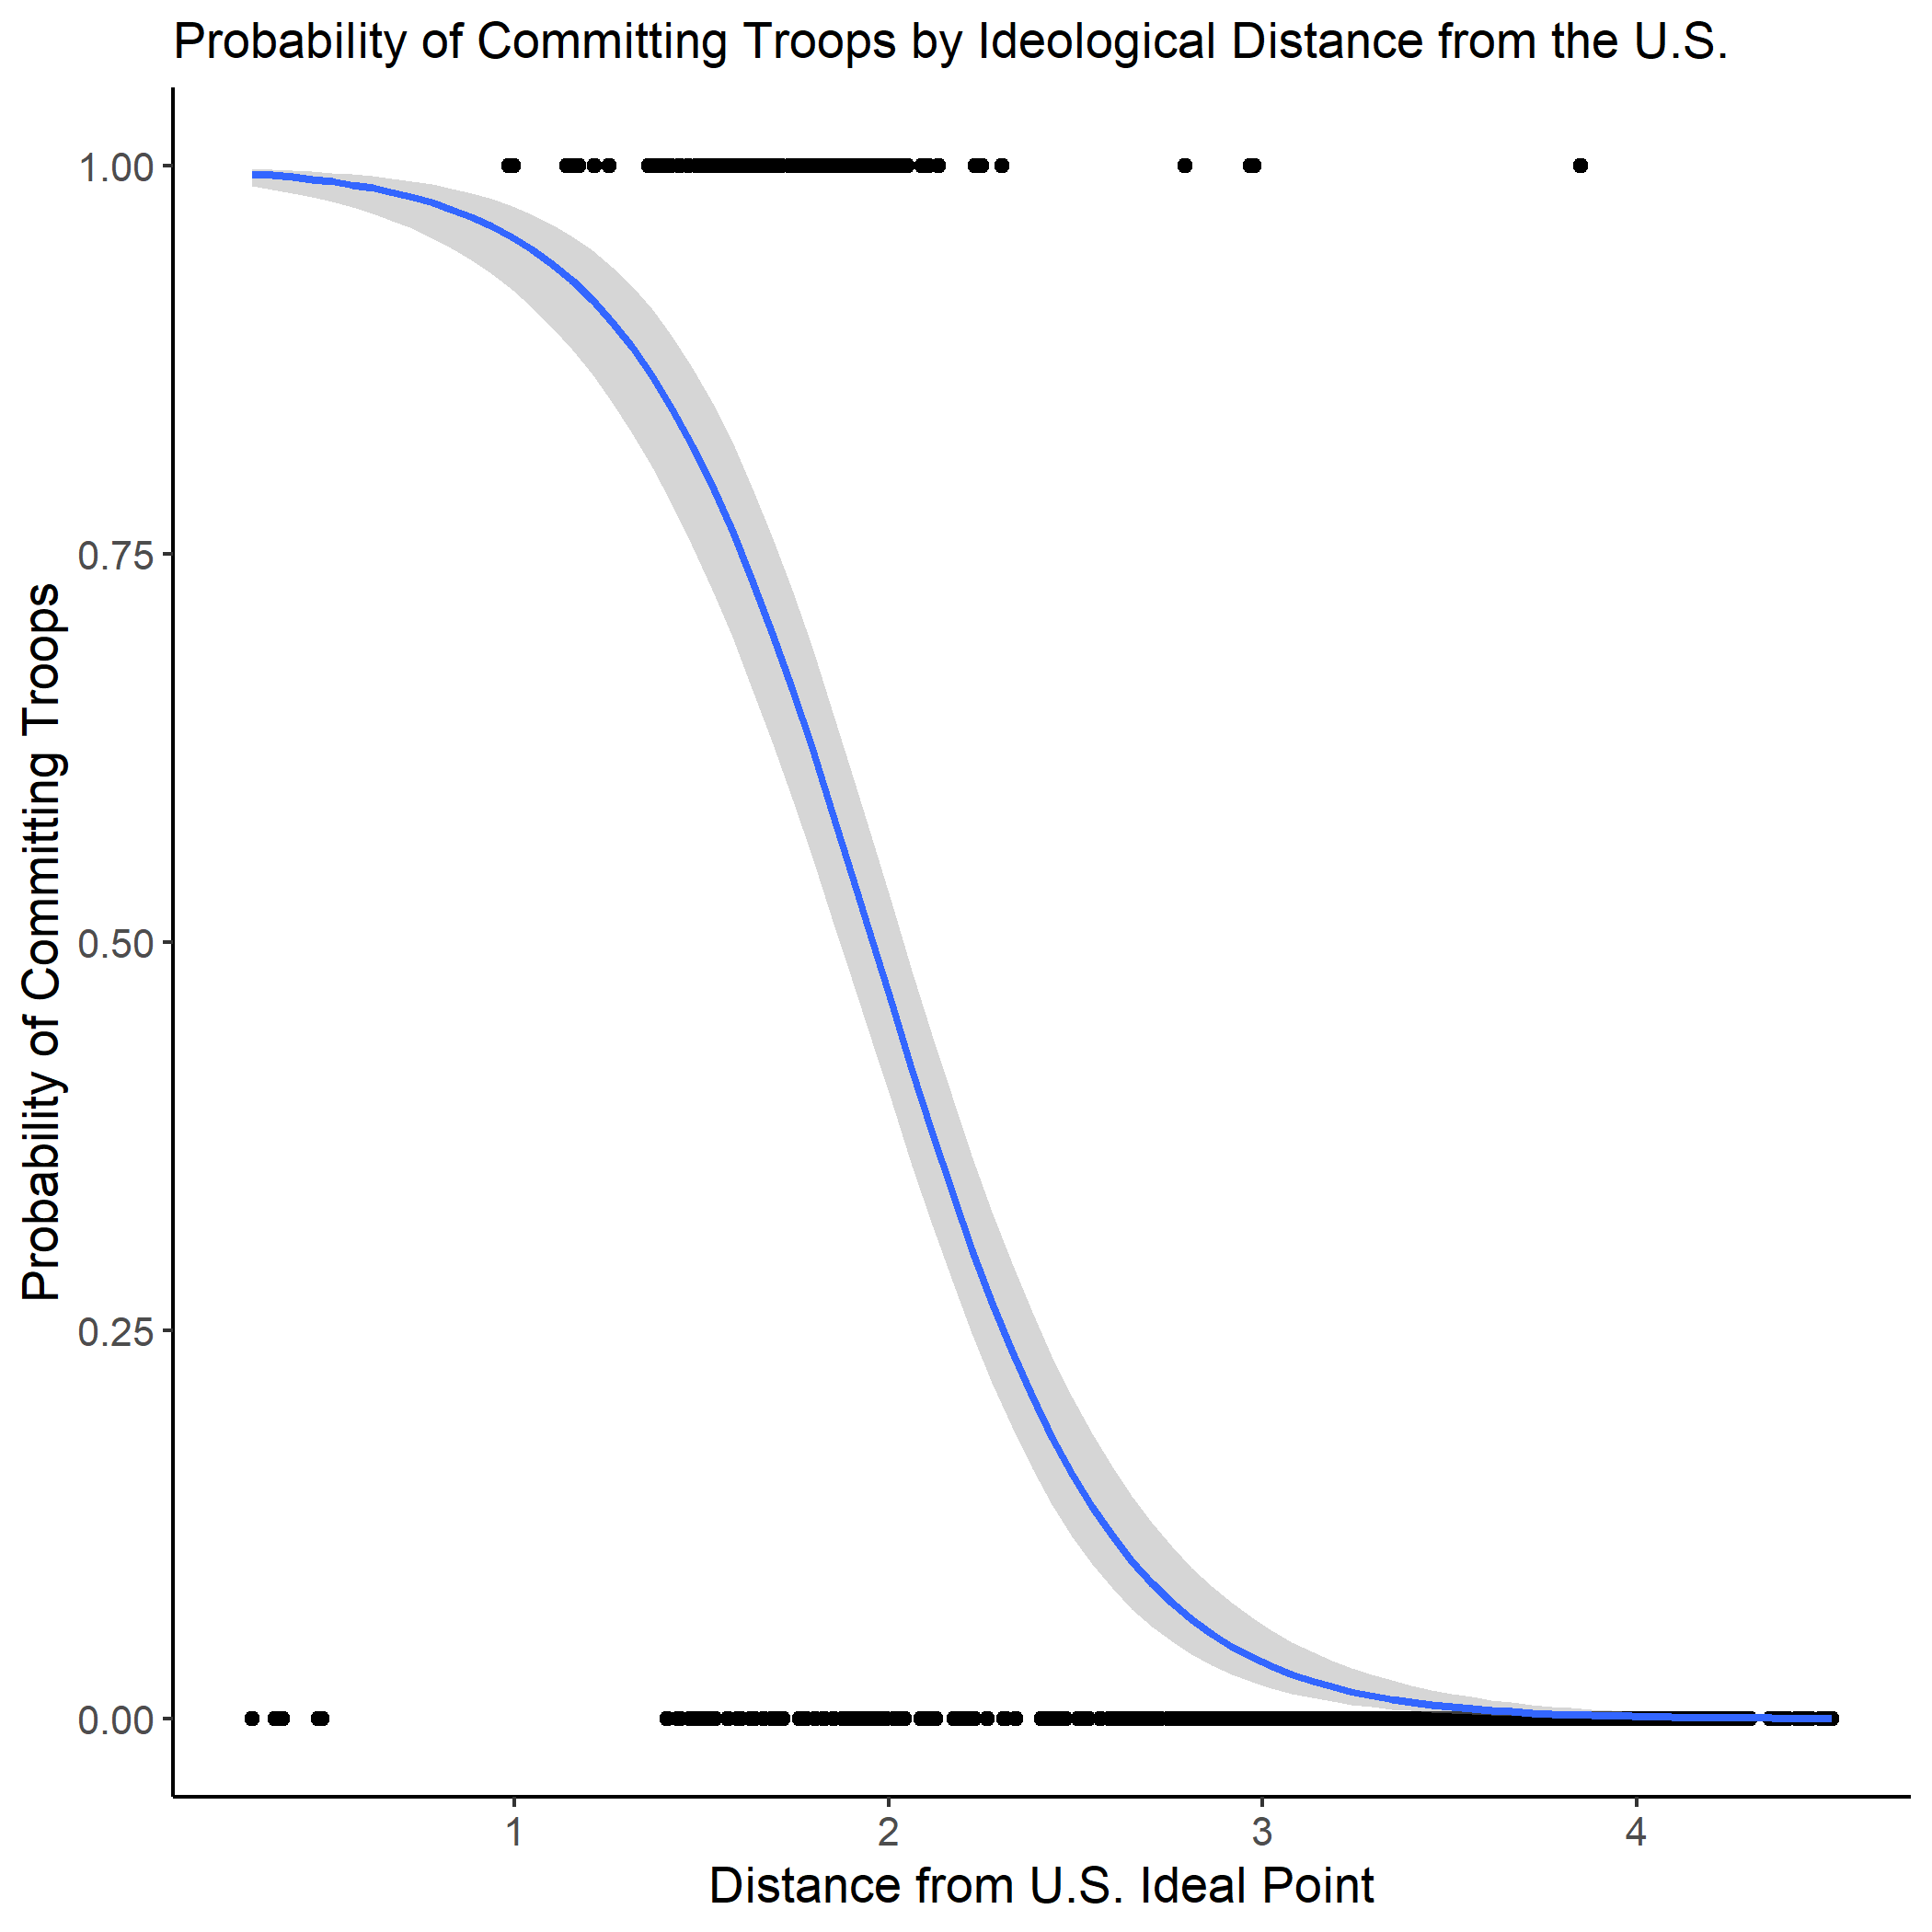
\includegraphics[width=0.65\textwidth]{figures/logit.png}
			\caption{Predicted probability of committing troops against actual decision}
			\label{fig:logit}
			\end{figure}

		\subsubsection{Model 2: Decision to Over-commit Troops}
			Next, we subset the data to only look at contributors and then examine the predictors of how many troops a country commits, relative to its available number of troops. Here our equations are almost the same, but we include a squared employ linear, as opposed to logistic, regressions because the dependent variable is continuous. With respect to the linear model, we avoid polynomial terms because they force the specified relationship onto the data, instead testing for the expected positive relationship if a linear model is fit.\footnote{Note that we expect strong ties to commit more than weak ties, meaning an expected positive slope.} After confirming these results we switch to a generalized additive model to explicitly capture non-linear effects.

			\vspace{-2em}
			\begin{equation*}
				\text{troop\_ratio}_{it} = \beta_0 + \beta_1\text{equiv}_{it} +
				\beta_2\text{ideology}_{it} + \beta_3\text{dem}_{it} + \beta_4\text{dist}_{it}
			\end{equation*}

			\begin{figure}[H]
			\centering
				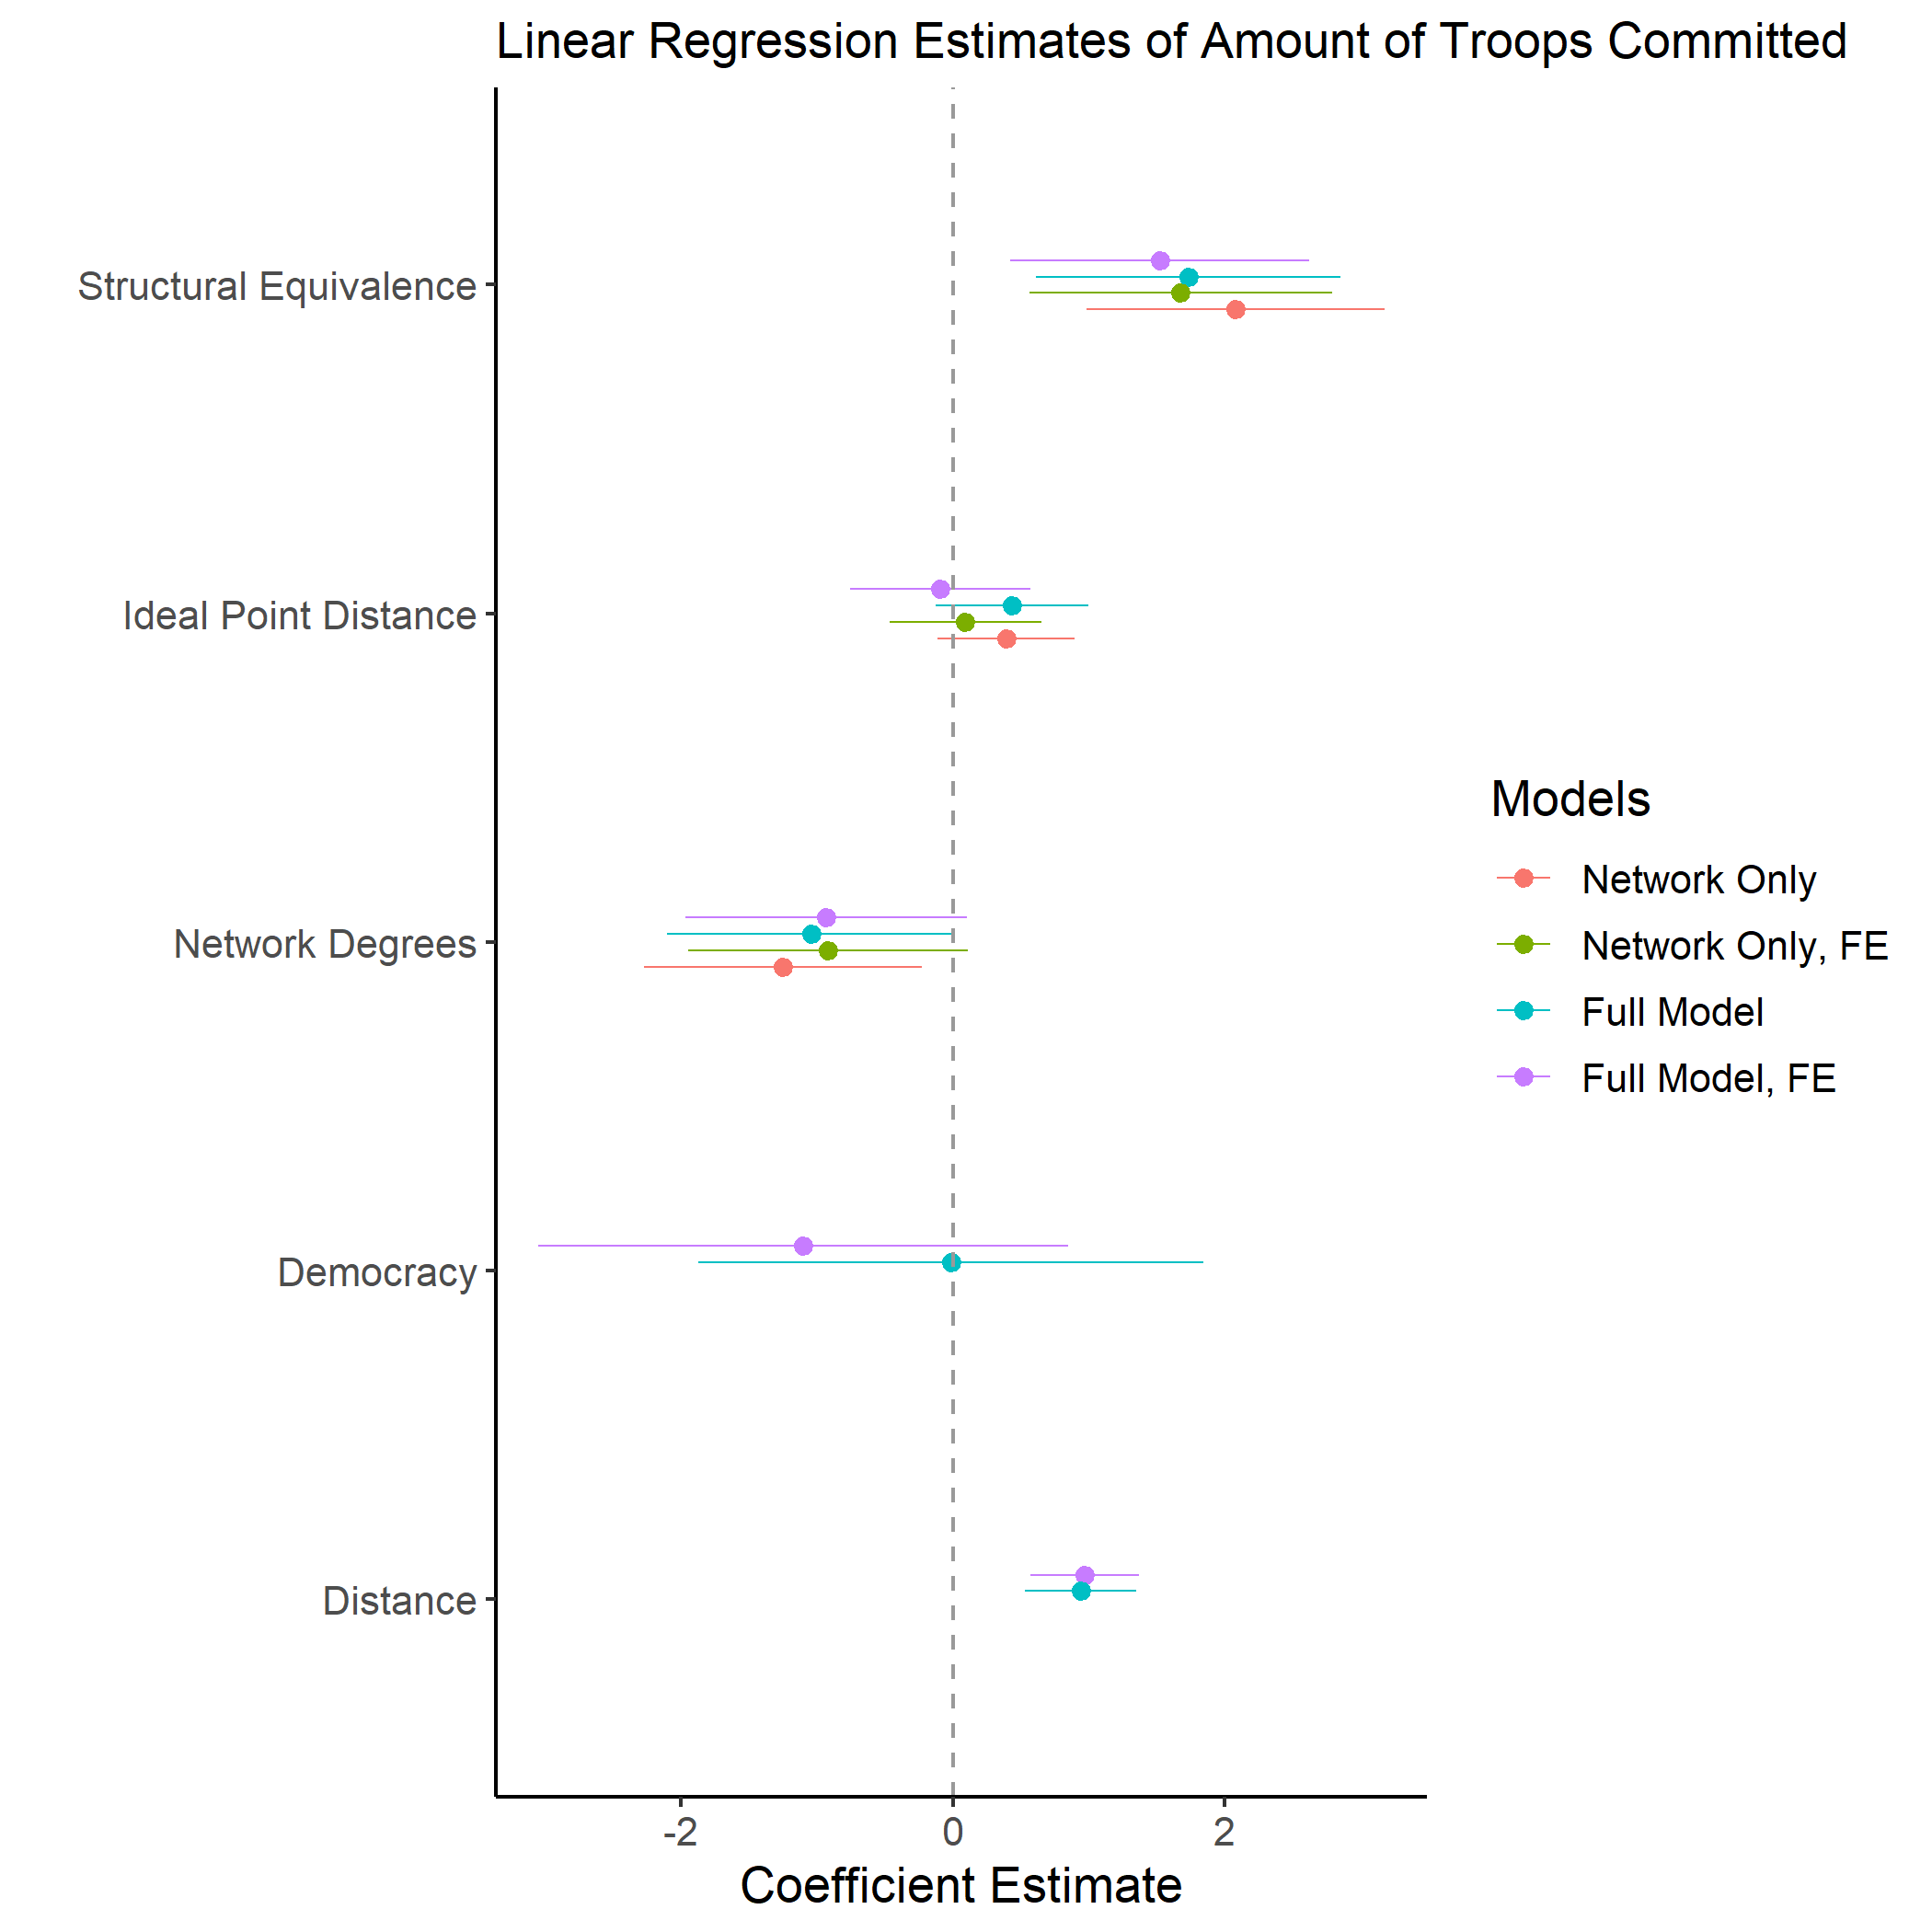
\includegraphics[width=0.725\textwidth]{figures/linear_coef.png}
			\caption{Model 2: Number of troops contributed, relative to number of available troops}
			\label{fig:linear_reg}
			\end{figure}

		Now that we are looking solely at the size of a state's contributions, we see that structural equivalence emerges clearly as the primary predictor. Though some of the largest contributors, such as New Zealand, sit on the periphery of the alliance network, the more deeply a state is embedded in the United States' security community, then the greater its expected contribution, on average. This fits generally with our expectation, where, even though the relationship is not perfectly linear, we expect states that are closely aligned with the initiating state to contribute more than than those weakly aligned.

		Interestingly, democracy is associated with a lower troop contribution than non-democracies. This actually aligns with work that has argued that that democracies are less reliable allies and more likely to pull out of coalition conflicts early \citep{massie_whydemocraticallies_2016, gartzke_whydemocraciesmay_2004}. While a slightly different context than our theory, these arguments provide a logical extension as to why we should expect that democracies may actually be less likely to over-contribute.


		Moving forward, we estimate a series of GAMs to test our core curvilinear hypothesis. GAMs are similar in structure to GLMs, but model relationships as a result of functions (which can be non-linear) rather than a constant coefficient. This generally takes the form of:

		\begin{equation*}
			f(x) = y_i = \alpha + f_1(x_{i1}) + f_2(x_{i2}) + ... + f_p(x_{ip}) + \varepsilon_i
		\end{equation*}

		where each function, $f_1, f_2, f_3, ..., f_p$ models the relationship between predictor and outcome, but can easily accommodate linear and non-linear effects.

		\begin{figure}[ht]
		\centering
		\begin{minipage}{.5\textwidth}
		  \centering
		  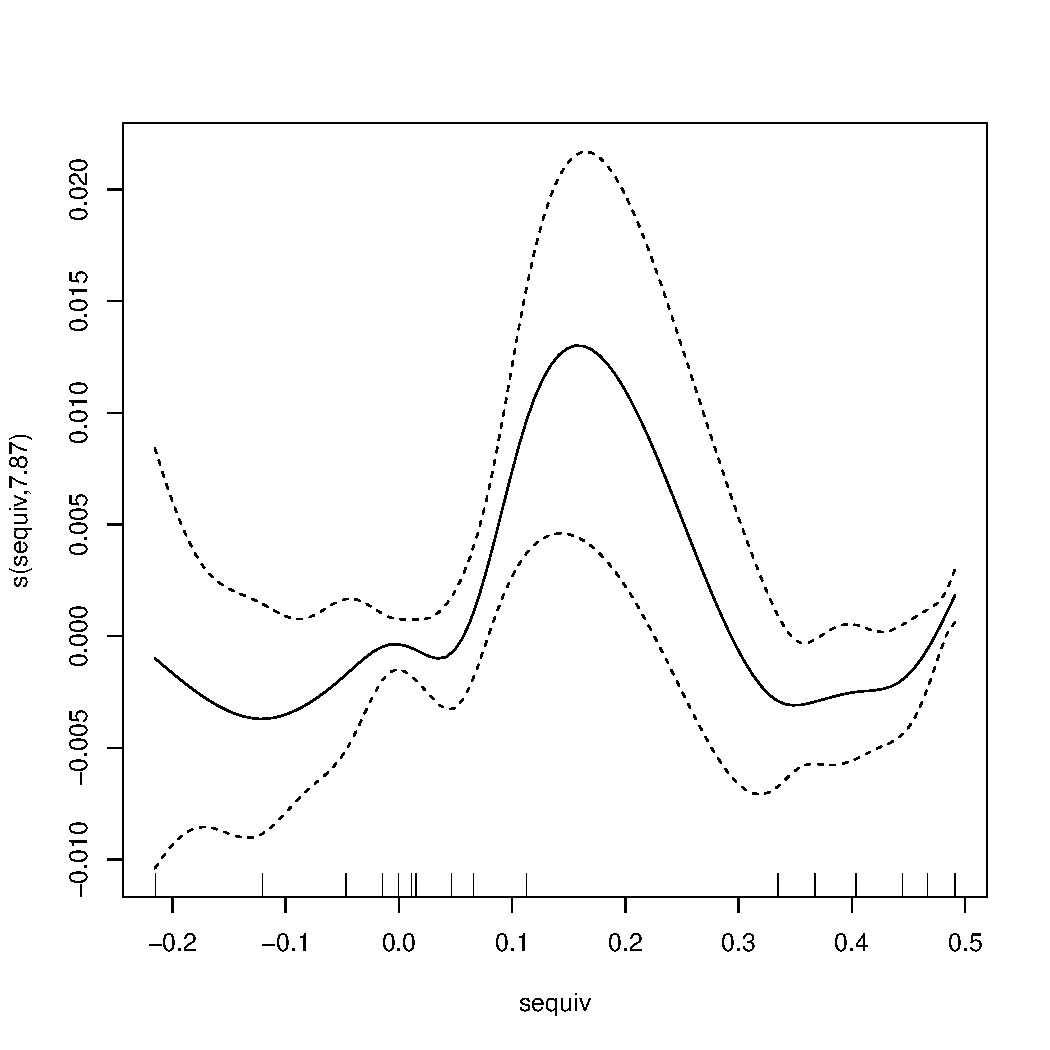
\includegraphics[width = \linewidth]{figures/no_can_gam.pdf}
		  \captionof{figure}{GAM without Canada}
		  \label{fig:test1}
		\end{minipage}%
		\begin{minipage}{.5\textwidth}
		  \centering
		  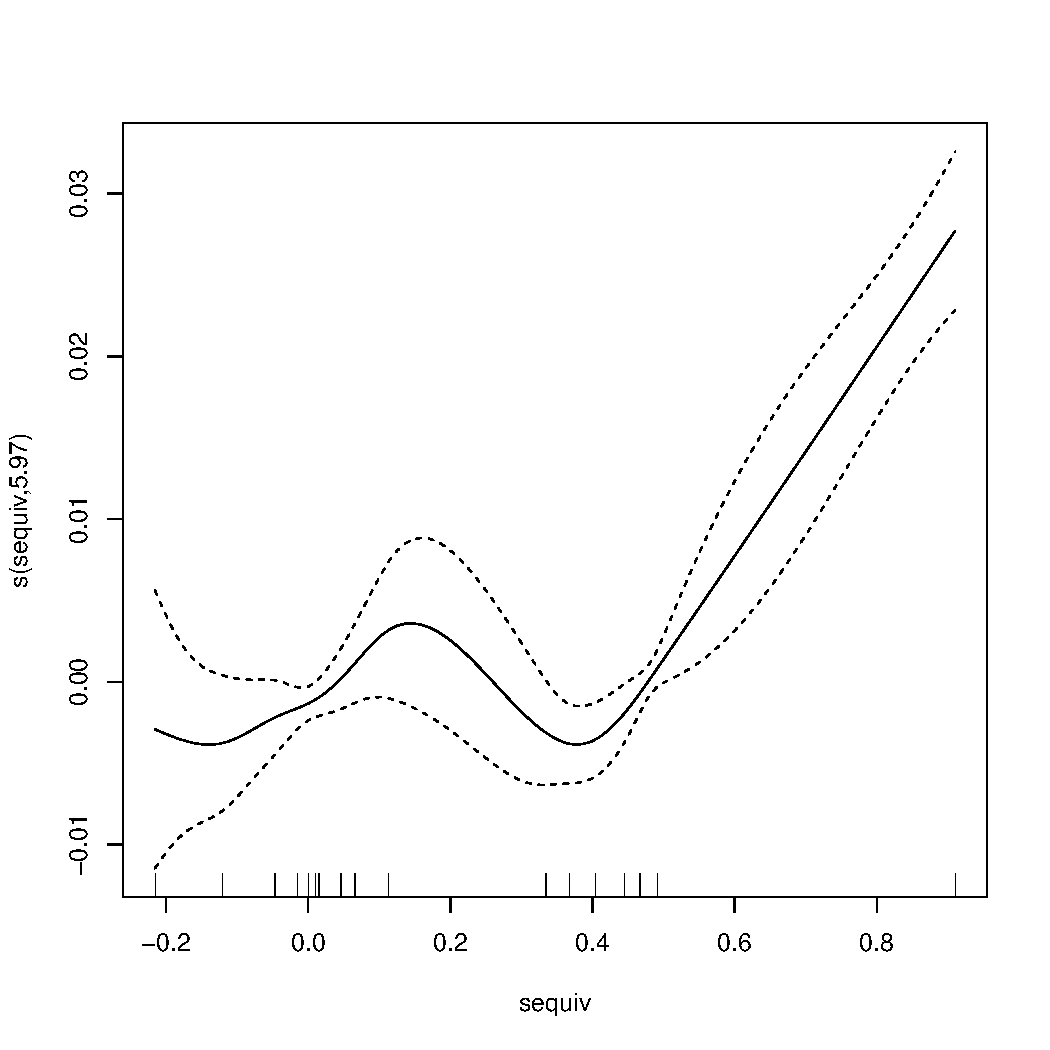
\includegraphics[width= \linewidth]{figures/can_gam.pdf}
		  \captionof{figure}{GAM including Canada}
		  \label{fig:test2}
		\end{minipage}
		\end{figure}

		Across both models -- with and without Canada -- we find that smoothing function is statistically significant and the function corresponds well to the hypothesis, with a non-linear curve corresponding to moderately structurally equivalent states.

\section{Discussion}
	Our findings runs counter to that expected by theories about the balance of threats. For the balance of threat hypothesis, the states with the highest contributions are those that are most concerned about the threat the opposing state presents to their security \citep{haesebrouck_democraticparticipationair_2016}. Yet, when contributions are measured as internal costs relative to the contribution a state could have made, the highest contributions are from states that appear to be opting into a war in which they have no material stake. Denmark, New Zealand, and Romania, 3 of the top 4 contributors to ISAF in 2001 by our measure, are not the states that are most concerned about the threat that the Taliban and Al Qaeda posed to their national security. This empirical observation is not explained by the theory that states enter an alliance in order to balance against threats \citep{walt_originsalliance_1987}.

	Our findings also contrast those who have tested domestic politics explanations in the context of the war in Afghanistan. NATO's formal institutional structure was supposed to render public opinion less relevant as an explanation for coalition participation \citep{kreps_eliteconsensusdeterminant_2010}. However, we find that while NATO membership and its accompanying obligations to avoid accusations of defection may be sufficient to explain why states do not free ride, that does not explain why states like New Zealand that are not bound by alliance obligations end up over-contributing.

	Previous theories described under the rubric of the alliance hypothesis also fail to explain this findings. For previous theories, ally support is expected when you can leverage your allies' power in your favor and is thus a measure of closeness \citep{davidson_neoclassicalrealistexplanation_2011}. This expects states that are the closest allies with the United States to be the largest contributors to US war efforts. Yet the relationship we see appears non-linear. These states do not over-contribute because the United States is their best protector or because they think they have the ability to influence the United States through their international clout as \citet{ringsmose_natoburdensharingredux_2010} finds. Rather, it is the states that want the United States to be their best protector or that \textit{want} the ability to influence international relations with the United States that are most likely to over-contribute. It's also not the case that the US coerced its closest allies into participating as argued by \citet{kupchan_natopersiangulf_1988} because those are not the states that ended up doing the most participating relative to what they could have contributed. Thus, desire for stronger ties and the expectation that over-contribution will positively signal that desire explains our findings in a way that differs from previous theories.

	While this analysis is limited to an examination of the war in Afghanistan, there is suggestive evidence that the theory holds for other coalition conflicts. During the war in Libya, Denmark make a concerted effort to over-contributed forces, particularly air forces to the bombing campaign, in order to demonstrates their ``relevance and trustworthiness to its great power allies in NATO, especially the United States" \citep{jakobsen_prestigeseekingsmallstates_2018, dicke_natoburdensharinglibya_2013}. This effort appears to have paid off. US Secretary of Defense Robert Gates commended Denmark for its costly contribution to the conflict when he publicly noted that Denmark ``...with their constrained resources, found ways to do the training, buy the equipment, and field the platforms necessary to make a credible military contribution."

\section{Conclusion}
	This paper suggest that the study of state contributions to coalition warfare provides unique insights if those contributions are measured relative to the cost they impose onto the contributor rather than the utility they provide regarding the conflict outcome. Not every state contributes to a war effort in order to influence the outcome of the war as theories of balance of threats predict. But it is also not the case, as predicted by the collective action hypothesis do states simply free ride when the conflict outcome is immaterial or, as predicted by the alliance dependence hypothesis, that the stronger your alliance, the more you contribute.

	Rather, because war is costly, it can serve as a signaling function for states that want to convey their desire to improve their relationship with other states in the international system. By accepting comparatively large costs to fighting alongside another state, especially when such fighting does not otherwise benefit you, states can signal how much they value an alliance relationship in a way that they anticipate generating reciprocity and payoffs down the road. Future work should examine whether states are making a smart bet in anticipating future payoffs from costly over-contributions; it is possible their gamble is incorrect. But for now, it suffices to say that states with the most interest in future payoffs from a better alliance relationship are the same states most likely to separate themselves from the rest of the coalition pact by over-contributing to wartime coalitions in the hopes that doing so signals their reliability.
	%that they are not a friend without benefits.


\section{Next Steps}

Below we include a few areas where we could use some feedback.

\begin{enumerate}

	\item Is structural equivalence the right measure of the strength of a tie?
		\begin{enumerate}
			\item It has been convenient and readers will likely be familiar, but it also is not exactly what we are aiming for. If two states have very similar networks, then they are not necessarily strong allies, though the probability they are seems to increase. Another option is to fit a latent space model of alliance tie formation \citep{hoff2002} and then use the estimated Euclidean distances as a measure of tie strength.
			\item We could also construct multiple networks (alliances, trade, diplomatic ties, arms trade) and use similarity across the multiplex network to construct a multidimensional strength of tie measure.
		\end{enumerate}
	\item Canada's outsized contributions:
			\begin{figure}[H]
			\centering
				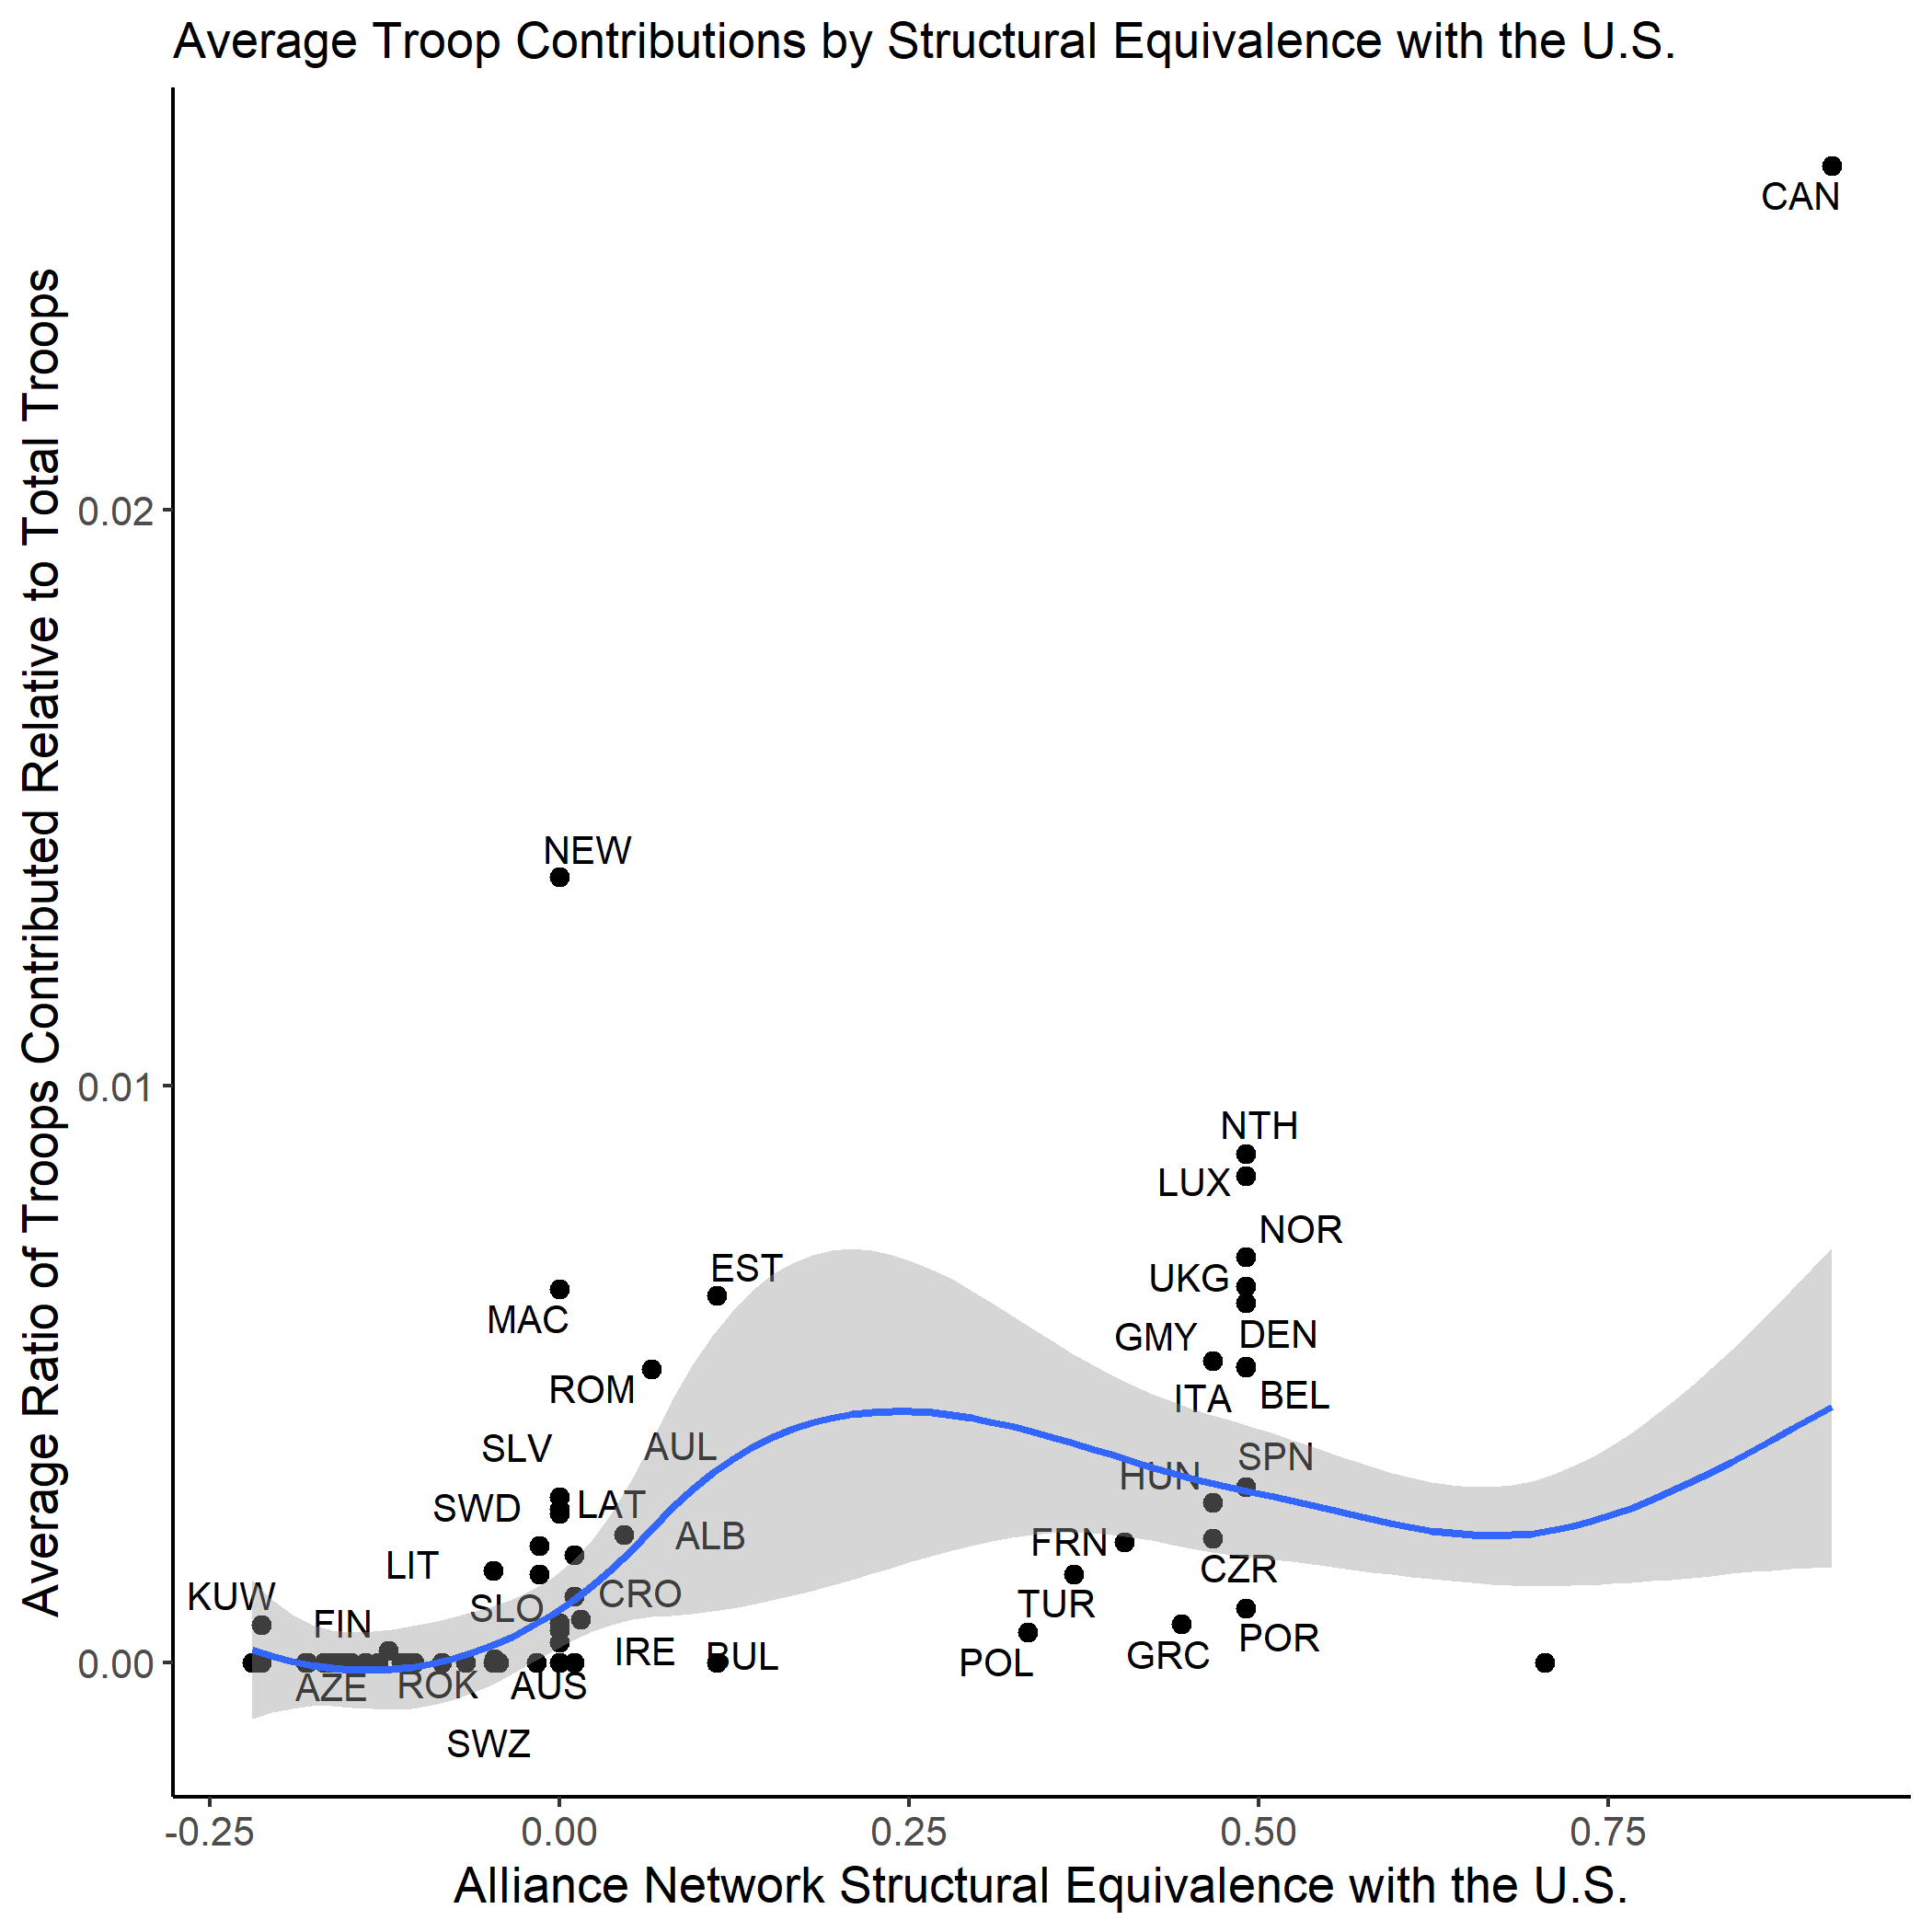
\includegraphics[width=0.55\textwidth]{figures/contributions_canada.png}
			\caption{Troop Ratio by Structural Equivalence with the United States}
			\label{fig:contr_sequiv_can}
			\end{figure}

		\begin{enumerate}
			\item Any thoughts on how to deal with this are appreciated.
		\end{enumerate}


	\item Next modeling steps:
	\begin{enumerate}
		\item Fit the model on 2001-2014 with Afghanistan, not just 2001-2005. But we need to deal with casualty aversion. Right now the plan is to just control for casualties on the right-hand side.
		\item We've received feedback to test the theory with the Iraq War. Though we haven't fit any models for Iraq yet, the data is almost ready and in identical format. So our plan is to finalize the empirical models for Afghanistan. treating it as a training set, and then we will test the models on Iraq. If the theory is accurate, then a model that captures the theory should have similar results -- not necessarily identical but similar in general relationship -- across conflicts. Iraq then will serve as a literal means of assessing out-of-sample performance.
	\end{enumerate}
\end{enumerate}


\bibliographystyle{apsr}
\bibliography{isaf_alliances}


\end{document}
